%!TEX root = ../thesis.tex
%******************************************************************************
\chapter{Introduction}\label{ch:introduction}
%******************************************************************************

Enterprise Systems like customer-billing systems or financial transaction systems are required to process large volumes of data in a fixed period of time. For example, a billing system for a large telecommunication provider has to process more than 1 million bills per day.
Those systems are increasingly required to also provide near-time processing of data to support new service offerings.

Traditionally, enterprise systems for bulk data processing are implemented as batch processing systems \citep{Fleck:1999aa}. Batch processing delivers high throughput but cannot provide near-time processing of data, that is the end-to-end latency of such a system is high. End-to-end latency refers to the period of time that it takes for a business process, implemented by multiple subsystems, to process a single business event.  For example, consider the following billing system of a telecommunications provider:
\begin{itemize}
	\item Customers are billed once per month
	\item Customers are partitioned in 30 billing groups
	\item The billing system processes 1 billing group per day, running 24h under full load.
\end{itemize}
In this case, the mean time for a call event to be billed by the billing system is 1/2 month. That is, the mean end-to-end latency of this system is 1/2 month.

\section{Systems for Bulk Data Processing}

\begin{figure}[h!tbp]
	\centering
	\mbox{\subfloat[Single processing line]{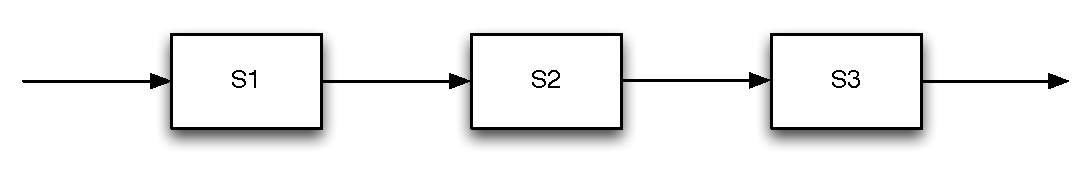
\includegraphics[width=\columnwidth]{considered_system_single}\label{fig:ch01_system_single}}}
	\mbox{\subfloat[Parallel processing lines]{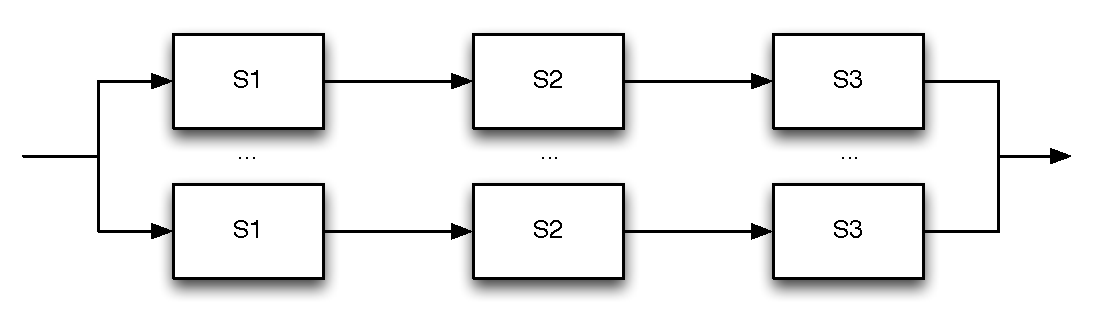
\includegraphics[width=\columnwidth]{considered_system_parallel}\label{fig:ch01_sytem_parallel}}}
	\caption{A system consisting of several subsystems forming a processing chain}
\end{figure}

A distributed system for bulk data processing considered in this research consists of several subsystems running on different nodes that together form a processing chain, that is, the output of subsystem S1 is the input of the next subsystem S2 and so on (see Figure \ref{fig:ch01_system_single}).

To facilitate parallel processing, the system can consist of several lines of subsystems with data beeing distributed among each line.

\subsection{An Example: Billing Systems for Telecommunications Carriers}
An example of a system for bulk data processing is a billing system of a telecommunications carrier. A billing system is a distributed system consisting of several sub components that process the different billing sub processes like mediation, rating, billing and presentment (see Figure \ref{fig:ch01_billing_process}).

The performance requirements of such a billing system are high. It has to process more than 1 million records per hour and the whole batch run needs to be finished in a limited timeframe to comply with service level agreements with the print service provider. Since delayed invoicing causes direct loss of cash, it has to be ensured that the bill arrives at the customer on time.

\begin{figure}[htbp]
	\centering
	
\includegraphics[width=\columnwidth]{billing_process}
	\caption{Billing process}
	\label{fig:ch01_billing_process}
\end{figure}

\subsection{Near-Time Processing of Bulk Data}
A new requirement for systems for bulk data processing is near-time processing. Near-time processing aims to reduce the end-to-end latency of a business process, that is, the time that is spent between the occurrence of an event and the end of its processing. In case of a billing system, it is the time between the user making a call and the complete processing of this call including mediation, rating, billing and presentment.

The need for near-time charging and billing for telecommunications carriers is induced by market forces, such as the increased advent of mobile data usage and real-time data services \citep{Cryderman:2011aa}. Carriers want to offer new products and services that require real-time or near-time charging and billing. Customers want more transparency, for example, to set their own limits and alerts for their data usage, which is currently only possible for pre-paid accounts. Currently, a common approach for carriers is to operate different platforms for real-time billing of pre-paid accounts and traditional batch-oriented billing for post-paid accounts. To reduce costs, carriers aim to converge these different plattforms.

A lower end-to-end latency can be achieved by using single-event processing, for example by utilizing a message-oriented middleware for the integration of the services that form the enterprise system. While this approach is able to deliver near-time processing, it is hardly capable for bulk data processing due to the additional communication overhead for each processed message. Therefore, message-based processing is usually not considered for building a system for bulk data processing requiring high throughput.

The processing type is usually a fixed property of an enterprise system that is decided when the architecture of the system is designed, prior to implementing the system. This choice depends on the non-functional requirements of the system. A system is therefore either optimized for low latency or high maximum throughput. 
These requirements are not fixed and can change during the lifespan of a system, either anticipated or not anticipated.

Additionally, enterprise systems often need to handle load peaks that occur infrequently. For example, think of a billing system with moderate load over most of the time, but there are certain events with very high load such as New Year's Eve. Most of the time, a low end-to-end latency of the system is preferable when the system faces moderate load. During the peak load, it is more important that the system can handle the load at all. A low end-to-end latency is not as important as an optimized maximum throughput in this situation.

\section{Aims and Objectives of the Research}\label{sec:research_objectives}
This research project aims to find a solution for the following problem:
\begin{quote}
\textbf{How to achieve high-performance near-time processing of bulk data?}
\end{quote}

Based on this problem, the thesis aims to answer the following research questions:
\begin{itemize}
	\item \textbf{RQ1:} What are the performance characteristics of batch and single-event processing systems?
	\item \textbf{RQ2:} What is the impact of data granularity on end-to-end latency and maximum throughput?
	\item \textbf{RQ3:} What is an appropriate middleware design that is able to miminize the end-to-end latency for different load scenarios?
	\item \textbf{RQ4:} What software processes are needed to design, implement and operate an adaptive system for near-time processing of bulk data?
\end{itemize}

To approach these research questions, the research project has the following key objectives:
\begin{enumerate}[label=\Alph*.]
	\item Performance evaluation of batch and messaging systems regarding maximum throughput and end-to-end latency.
	\item Development of a concept for an adaptive middleware that delivers low latency while providing high throughput.
	\item Implementation of a research prototype used for demonstrating the practicability of the concept.
	\item Specification and conduction of appropriate performance tests to evaluate the developed approach.
	\item Development of a conceptional framework containing guidelines and rules for the practitioner how to implement an enterprise system based on the adaptive middleware for near-time processing of bulk data.
\end{enumerate}

\section{Research Methodology}
An evaluation of current approaches to optimize the performance of service-oriented systems has been conducted to get an understanding of the field and the involved problems.

To better understand the performance characteristics of batch and message-based single-event processing two prototypes of each processing style has been implemented. Using these prototypes, a performance evaluation has been done to better understand the differences between the two processing styles, with a special focus on the end-to-end latency and maximum throughput. The message-based prototype has been extended to study the impact of data granularity on end-to-end latency and maximum throughput.

Based on the results of the performance evaluation of the batch and message-based prototype, the concept of an adaptive middleware has been developed. The message-based prototype has been extended to implement the concepts of the adaptive middleware. Using this prototype, a performance evaluation has been conducted to evaluate the proposed concepts for an adaptive middleware for bulk data processing.

\newpage

\section{Contributions}\label{sec:contributions}
This thesis makes the following contributions to the field:

\begin{itemize}
	\item \textbf{A Performance evaluation of batch and messaging systems regarding maximum throughput and end-to-end latency}\\\\
	The performance evaluation compares the performance of batch and message-based systems. It analyses the impact of different processing styles, that is batch and message-based processing, on throughput and latency. It shows that throughput and latency of a messaging system depend on the level of data granularity and that the throughput can be increased by increasing the granularity of the processed messages.
	\item \textbf{A concept and prototype implementation of a feed\-back-con\-trolled adaptive middleware for near-time processing of bulk data}\\\\
	The adaptive middleware is able to adapt its processing type fluently between batch processing and single-event processing. By using message aggregation, message routing and a closed feedback-loop to adjust the data granularity at runtime, the system is able to minimize the end-to-end latency for different load scenarios.
	\item \textbf{A Conceptual Framework to Guide the Development of Feed\-back-Controlled Bulk Data Processing Systems}\\\\
	The design, implementation and operation of an adaptive system for bulk data processing differs from common approaches to implement enterprise systems.
	The conceptual framework describes the development process of how to build an adaptive software for bulk data processing. It defines the needed roles and their skills, the necessary tasks and their relationship, artifacts that are created and required by different tasks, the tools that are needed to process the tasks and the processes, which describe the order of tasks.
\end{itemize}

\section{Outline of the Thesis}\label{sec:thesis_outline}

The thesis is organized as follows:

\begin{enumerate}
	\item \textbf{Introduction}\\\\
	This chapter sets the context for the conducted research. It specifies the aims and objectives and methodology of this research, followed by a brief description of the contributions. 
	\item \textbf{Background}\\\\
	This chapter further defines the context of this research and introduces core concepts and terms that are used throughout the thesis. It starts with an introduction to batch and message-based processing paradigms and analyzes the relationship between maximum throughput and end-to-end latency. Additionally, it describes performance issues of an \ac{SOA} middleware and discusses current approaches for performance optimizations of such a middleware.
	\item \textbf{Related Work}\\\\
	This chapter describes related work and demarcates it to the work of the research presented in this thesis. It starts with a summary of work related to the performance of service-oriented systems and approaches for performance optimizations. The chapter introduces the concept of self-adaptive software and presents related work in the context of self-adaptive middleware.
	\item \textbf{Performance Evaluation of Batch and Message-based Systems}\\\\
	This chapter compares the performance of a batch and message-based system. It introduces the batch and message-based prototype systems that have been imple- mented and describes the performance evaluation to compare the performance characterics of the two different processing types.  The impact of data granularity on throughput and latency of the messaging prototype is evaluated and discussed. In addition, the chapter gives an overview of other work related to the content of this chapter.
	\item \textbf{An Adaptive Middleware for Near-Time Processing of Bulk Data}\\\\
	This chapter presents the design, implementation and evaluation of the adaptive middleware which is able to adapt its processing type fluently between batch processing and single-event processing. It starts with a description of the core concepts, such as message aggregation, message routing, and monitoring and control, followed by a discussion of important design aspects such as service design, transports, error handling and controller design.
	The design and implementation of a prototype of the adaptive middleware is outlined. A performance evaluation of the prototype is described. It is shown that the concept of an adaptive middleware for bulk data processing is able to minimize the end-to-end latency of a system. Additionally, the chapter gives an overview of other work related to feedback-control of computing systems.
	\item \textbf{A Conceptual Framework to Guide the Development of Feed-back-Controlled Bulk Data Processing Systems}\\\\
	This chapter presents a framework that guides the practitioner to design, implement and operate a system based on the adaptive middleware for bulk data processing. It starts with a description of the metamodel of the framework, followed by a description of the entities of the process model, such as phases, roles, tasks, artifacts and tools. It is discussed how the conceptual framework can be used with other software development methodologies. The chapter gives an overview of other work related to the content of this chapter.
	\item \textbf{Conclusion}\\\\\
	This chapter concludes the thesis with a summary of the key objectives and contributions. It discusses the limitations of this research and identifies future work.
\end{enumerate}